
\section{Background}
\label{sec:background}

\subsection{Class-incremental learning}
\label{sec:cil}

\begin{figure}[h]
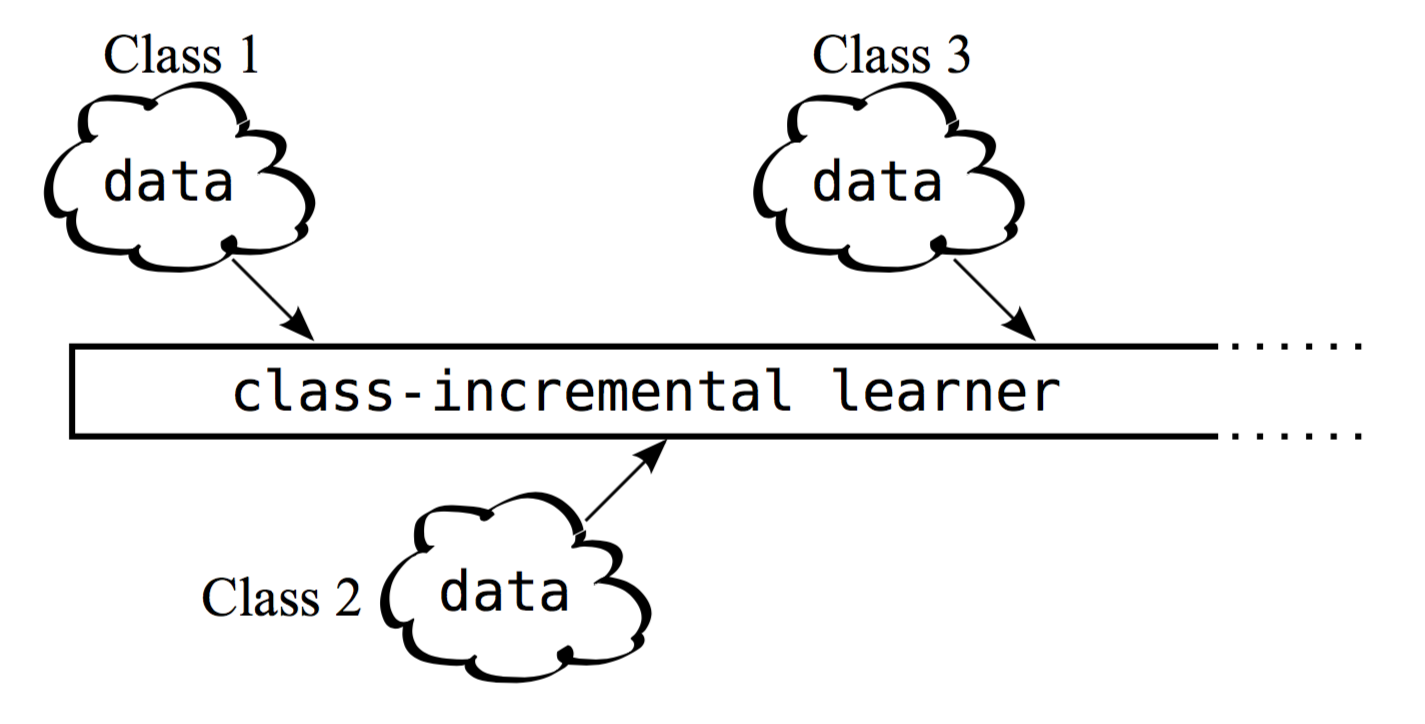
\includegraphics[width=80mm]{data/class-incremental_learning.png}
\centering
\caption{Class-incremental learning: an algorithm learns continuously from a sequential data stream in which new classes occur. At any time, the learner can perform multi-class classification for all classes observed so far. \label{fig:class-incremental_learning}}
\end{figure}

There are three formal properties of an algorithm to qualify as class-incremental:
\begin{enumerate}
\item it should be trainable from a stream of data in which examples of different classes occur at different times,
\item it should at any time provide a competitive multi-class classifier for the classes observed so far,
\item its computational requirements and memory footprint should remain bounded, or at least grow very slowly, with respect to the number of classes seen so far.
\end{enumerate}
The first and second properties directly express the essence of Class-Incremental Learning. The third criterion concerns about practicality and prevents trivial algorithms; the algorithms such as storing all training examples and retraining an ordinary classifier whenever new data arrives is meaningless.


\subsection{iCaRL: Incremental Classifier and Representation Learning}
\label{sec:icarl}

\begin{algorithm}[ht]
  \Input{$X^s, ..., X^t$ \Comment*[f]{training examples in per-class sets}}  
  \Input{$K$ \Comment*[f]{memory size}}  
  \Require{$\Theta$ \Comment*[f]{current model parameters}}
  \Require{$\mathcal{P} = \left(P_1, ..., P_{s-1} \right)$ \Comment*[f]{current exemplar sets}}
  $\Theta \leftarrow \textsc{UpdateRepresentation}\left(X^s, ..., X^t;\mathcal{P};\Theta\right)$ \\
  $m \leftarrow K/t$ \Comment*[f]{number of exemplars per class} \\
  \For {$y = 1..s-1$}{
    $P_y \leftarrow \textsc{ReduceExemplarSet}\left(P_y,m\right)$ 
  }
  \For {$y = s..t$}{
    $P_y \leftarrow \textsc{ConstructExemplarSet}\left(X_y,m,\Theta\right)$ 
  }
  $\mathcal{P} \leftarrow \left(P_1, ..., P_t\right)$ \Comment*[f]{new exemplar sets} \\
\caption{ iCaRL \textsc{IncrementalTrain} \label{alg:icarl_learn}}
\end{algorithm}


iCaRL~\cite{Rebuffi:2016aa}, an incremental classifier and representation learning, provides a practical strategy for simultaneous learning of classifiers and a feature representation in the class-incremental setting. Algorithm~\ref{alg:icarl_learn} shows the overall process of the training step of iCaRL.

There are three main components in its strategy to fulfill the criteria of Class-Incremental Learning. These three components are:

\begin{itemize}
  \item classification by a \textit{nearest-mean-of-exemplars} rule,
  \item \textit{prioritized exemplar selection} based on herding,
  \item representation learning using \textit{knowledge distillation} and \textit{prototype rehearsal}.
\end{itemize}

iCaRL learns classifiers and feature represeantation simultaneously from on a data stream in class-incremental form, \textit{i.e.} sample sets $X^1, X^2, ...$, where all examples of a set $X^y = \left\{ x_1^y, ..., x_{n_y}^y \right\}$ are of class $y \in \mathbb{N}$.

\subsubsection{Classification}
\label{sec:icarl_classification}

iCaRL relies on \textit{exemplar images} sets $P_1, ..., P_t$ that it select dynamically out of the data stream for each observed class so far. iCaRL ensures that the total number of exemplar images never exceeds a fixed parameter $K$. Therefore, the network's prediction rule is equivalent to the use of a linear classifier with non-linear feature map $phi$ and weight vectors $w_1, ..., w_t$.

\begin{algorithm}[ht]
  \Input{$x$ \Comment*[f]{image to be classified}}  
  \Require{$\mathcal{P} = \left(P_1, ..., P_t \right)$ \Comment*[f]{class exemplar sets}}
  \Require{$\phi : \mathcal{X} \rightarrow \mathbb{R}^d$ \Comment*[f]{feature map}}
  \For {$y = 1, ..., t $}{
    $\mu_y \leftarrow \frac{1}{\left| P_y \right|} \sum\limits_{y \in P_y} \phi\left( p \right)$ \Comment*[f]{mean-of-exemplars}
  }
  $y^{*} \leftarrow \underset{y = 1, ..., t}{\textrm{argmin}} \left\| \phi(x) - \mu_y \right\|$ \Comment*[f]{nearest prototype} \\
  \Output{class label $y^{*}$}
  
\caption{ iCaRL \textsc{Classify} \label{alg:icarl_classify}}
\end{algorithm}

Algorithm~\ref{alg:icarl_classify} describes the mean-of-exempars classifier. To predict a label, $y^*$, for a new image, $x$, it computes a prototype vector for each class observed so far, $\mu_1, ..., \mu_t$, where $\mu_y = \frac{1}{\left| P_y \right|} \sum_{y \in P_y} \phi\left( p \right)$ is the average feature vector of all exemplars for a class $y$. The class label whose prototype vector is the most similar with $x$ is assigned to $y^*$

\subsubsection{Representation Learning}
\label{sec:icarl_learning}

Whenever iCaRL gets data, $X^s, ..., X^t$ for new classes, $s, ..., t$, it updates its features extraction routine and the exemplar set. Algorithm~\ref{alg:icarl_update} lists the step for incrementally improving the feature representation. It mainly aims to prevent or at least mitigate \textit{catastrophic forgetting}~\cite{McCloskey:1989aa}, which is a deterioration of classification accuracy. It augmented the training set so that it consists not only of the new training examples but also of the stored exemplars. The lass function is augmented, too. It contains both the standard classification loss, which encourages improvements of the feature representation that allow classifying the newly observed classes, and the distillation loss, which ensures that the discriminative information learned previously is not lost during the new learning step.

\begin{algorithm}[ht]
  \Input{$X^s, ..., X^t$ \Comment*[f]{training images of classes $s, ..., t$}}
  \Require{$\mathcal{P} = \left( P_1, ..., P_{s-1}\right)$ \Comment*[f]{exemplar sets}}
  \Require{$\Theta$ \Comment*[f]{ current model parameters}}

  $\mathcal{D} \leftarrow \bigcup\limits_{y=s..t}\left\{ (x,y) : x \in X^y \right\} \cup \bigcup\limits_{y=1..s-1}\left\{ (x,y) : x \in P^y \right\} $ \Comment*[f]{form combined training set} \\
  \For{$y = 1, ..., s-1$}{ 
    $q_i^y \leftarrow g_y(x_i) \forall (x_i,\cdot) \in \mathcal{D}$ \Comment*[f]{store network outputs with pre-update parameters} \\
  } 
$l(\Theta) = - \sum\limits_{\left(x_i,y_i\right) \in \mathcal{D}} \left[ \sum\limits_{y=s}^t \delta_{y=y_i}\log g_y(x_i) + \delta_{y\neq y_i}\log \left(1-g_y(x_i)\right) + \sum\limits_{y=1}^{s-1} q_{i}^y\log g_y(x_i) + (1-q_i^y)\log \left(1-g_y(x_i)\right) \right]$ \Comment*[f]{run network traniing (\textit{e.g.} BackProp) with loss function that consists of \textit{classification} and \textit{distillation} terms.}

\caption{ iCaRL \textsc{UpdateRepresentation} \label{alg:icarl_update}}
\end{algorithm}

\subsubsection{Exampler Management}
\label{sec:icarl_exemplar}

\begin{algorithm}[ht]
  \Input{image set $X= \{x_1, ..., x_n\}$ of class $y$}
  \Input{$m$ target number of exemplars}
  \Require{current feature function $\phi : \mathcal{X} \rightarrow \mathbb{R}^d$}

  $\mu \leftarrow \frac{1}{n}\sum\limits_{x\in X} \phi(x)$ \Comment*[f]{current class mean} \\
  \For{$k = 1, ..., m$}{
    $p_k \leftarrow \underset{x \in X}{\textrm{argmin}} \left\| \mu - \frac{1}{k}\left[ \phi(x) + \sum\limits_{j=1}^{k-1} \phi(p_j) \right] \right\|$
  }
  $P \leftarrow (p_1, ..., p_m)$

  \Output{exemplar set $P$}
\caption {iCaRL \textsc{ConstructExemplarSet} \label{alg:icarl_exemplar_set}}
\end{algorithm}

Whenever iCaRL constructs exemplar sets for each classes, it treats all classes equally; iCaRL will use $m - K/t$ exemplars for each classes when it has been observed $t$ classes and the budget of the total number of the exemplars is $K$.

Algorithm~\ref{alg:icarl_exemplar_set} describes the exemplar selection step. The top $m$ exemplars, whose average feature vector over all exemplars best approximates the average feature vector over all training examples, are chosen. The reduction step is simple; on the sorted exemplars by aforementioned criterion, one discards the exemplars from the back until it reaches to desire size.

